\newpage
\section{Durchführung}
\label{sec:Durchführung}

\begin{figure}[htb]
  \centering
  \includegraphics[width=10.0cm]{pictures/Würfel.pdf}
  \caption{Würfelüositionen und der schematische Strahlenverlauf für die Messungen.}
  \label{fig:wuerfel}
\end{figure}

\begin{figure}[htb]
  \centering
  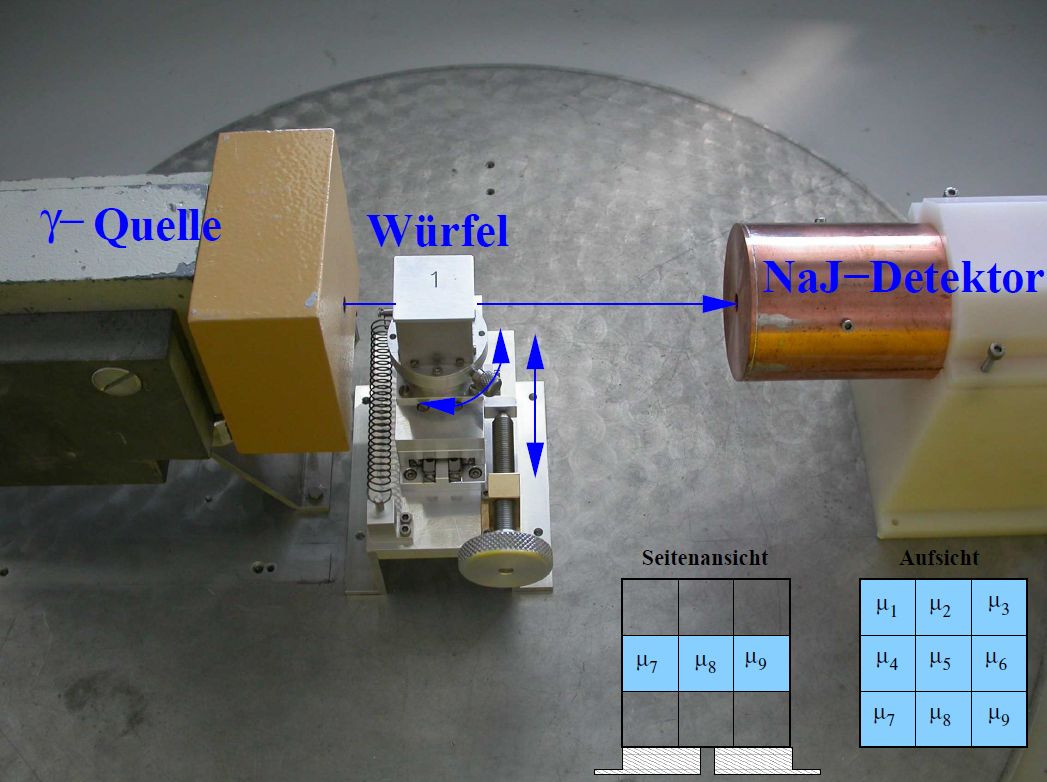
\includegraphics[height=7.0cm]{content/pictures/Aufbau.png}
  \caption{Darstellung des verwendeten Versuchsaufbaus.\cite{anleitung}}
  \label{fig:Aufbau}
\end{figure}
Zu Beginn des Versuchs wird der $\ce{^137Cs}$-Strahler durch den Assistenten, in den Versuchsaufbau aus Abbildung \ref{fig:Aufbau} eingebaut. 
Anschließend wird eine Nullmessung, dass bedeutet keine Probe im Strahlengang
aufgenummen. Dazu wird das Programm \textit{Maestro} verwendet, welches auf dem bereitgestellten Computer installiert ist.
Anschließend wird nur ein Aluminiumgehäuse, welches die Würfel im Inneren zusammen hält vermessen. Dabei ist darauf zu achetn, dass für einen statistischen Fehler
von weniger als \SI{3}{\percent} eine Zählrate von \num{1112} erreicht werden muss, was sich nach der Poissonverteilung ergibt. Es werden insgasamt
zwölf Messungen mit einem Strahlenverlauf wie in Abbildung \ref{fig:wuerfel} dargestellt, durchgeführt.
Nun werden noch zwei Vollwürfel untersucht, welche ebenfalls durch ein Aluminumgehäuse geschützt sind. Dazu werden für beide nur vier Messungen benötigt,
da die jeweils anderen äquivalent sind.
Zuletzt wird noch ein Würfel, welcher aus \num{27} Einzelwürfeln besteht genauer untersucht. Der Aufbau lässt aber nur die Vermessung der mittleren Ebene zu, hier werden 
wieder alle zwölf Messungen durchgeführt.
\FloatBarrier